\documentclass[12pt]{article}

\usepackage{graphicx}
\usepackage{wrapfig}
\usepackage{subfig}
\usepackage[T1,hyphens]{url}
\usepackage{hyperref}
\hypersetup{
    colorlinks=true,
    linkcolor=blue,
    filecolor=magenta,
    urlcolor=cyan,
}
\urlstyle{same}
\usepackage{float}

%------------------------------------------------%
%------------------------------------------------%
%------------------------------------------------%


\title{Two Sigma Data Challenge Report}
\author{Ben Jakubowski}
\date{\today}

\begin{document}
\maketitle

\section{Introduction}

For my project for the Two Sigma data challenge, I chose to use CitiBike trip data, plus external NOAA daily weather data, to build a predictive model of the number of CitiBike trips taken per day from 2014-2016. This modeling task is motivated by the assumption that the CitiBike system needs to regularly take bikes out of circulation for maintenance. If demand can be forecasted accurately, CitiBike may be able to predict dates with low demand and chose those days to take bikes out of circulation for maintenance.\\

In constructing my models, I made a number of assumptions:

\begin{itemize}
\item Bike trips are logged one week after the trip start date. This seems to be a very conservative assumption (and if more information were available on data availability, new lag features could be tested).
\item Weather predictions are essentially the same as actual weather conditions. This is a very liberal assumption, but actual weather condition data was available through a NOAA API, and (given time constraints for this project) robust datasets on past weather forecasts were not found. With additional time, the model would ideally be retrained on weather forecasts (with the appropriate time delta to account for this use case).
\end{itemize}

\section{Data}

I used two data sources to complete this project.
\begin{itemize}
\item CitiBike trip data. Available at \url{https://s3.amazonaws.com/tripdata/index.html}
\begin{itemize}
	\item The only feature computed from this dataset was the number of trips taken on each day from 01/01/2014-12/31/2016.
\end{itemize}
\item NOAA Climate Data Online. The API is documented at \url{https://www.ncdc.noaa.gov/cdo-web/webservices/v2}. Features taken from this datasource include:
\begin{itemize}
    \item Precipitation
    \item Snowfall
    \item Snow depth
    \item Max temperature
    \item Min temperature
    \item Average daily wind speed
    \item Fastest 2-minute wind speed
    \item Fastest 4-second wind speed
    \item (Binary): Fog, ice fog, or freezing fog (may include heavy fog)
    \item (Binary): Smoke or haze
\end{itemize}
\end{itemize}

In addition to raw features, a number of additional features were constructed for each day, including
\begin{itemize}
\item A day number feature (where $t_{\begin{tiny}\textrm{01/01/2014}\end{tiny}} = 0,~t_{\begin{tiny}\textrm{01/02/2014}\end{tiny}}= 1,~\cdots$). This feature was constructed under the hypothesis that the CitiBike system is relatively new, and probably has been growing (linearly) with time.
\item Trig features ($sin\left(\frac{2\pi t}{365.25}\right)$ and $cos\left(\frac{2\pi t}{365.25}\right)$) to capture hypothesized annual cycle in usage. Note these features were constructed with fixed one-year frequencies.
\item Average daily trip count over a 7-day window ending a week earlier.
\item Day of the week
\item Month number (to account for potential misspecification in the fixed seasonal cycle).
\end{itemize}

\section{Modeling}

First, we used a 90-10 training test split. Then two models were learned over the training set. The first (our baseline model) was an unregularized linear model including only $t$, $sin$, and $cos$ features (plus an intercept). The fit model is plotted below, along with the residual.

\begin{figure}[H]
   \centering
   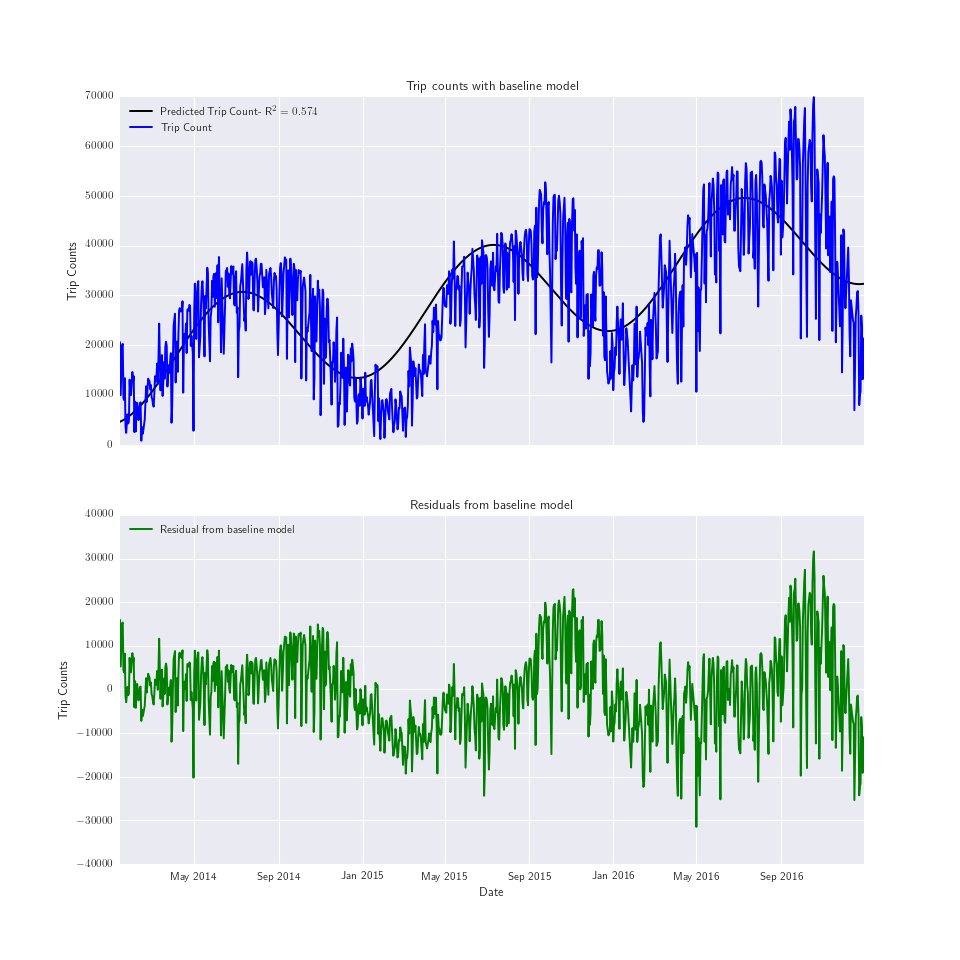
\includegraphics[width=\textwidth]{figures/baseline_plot.png}
  \end{figure}

Next, 5-fold cross validation was used to optimize ElasticNet hyperparameters for linear model including all the features. The final fit model is plotted below, along with the residual.

\begin{figure}[H]
   \centering
   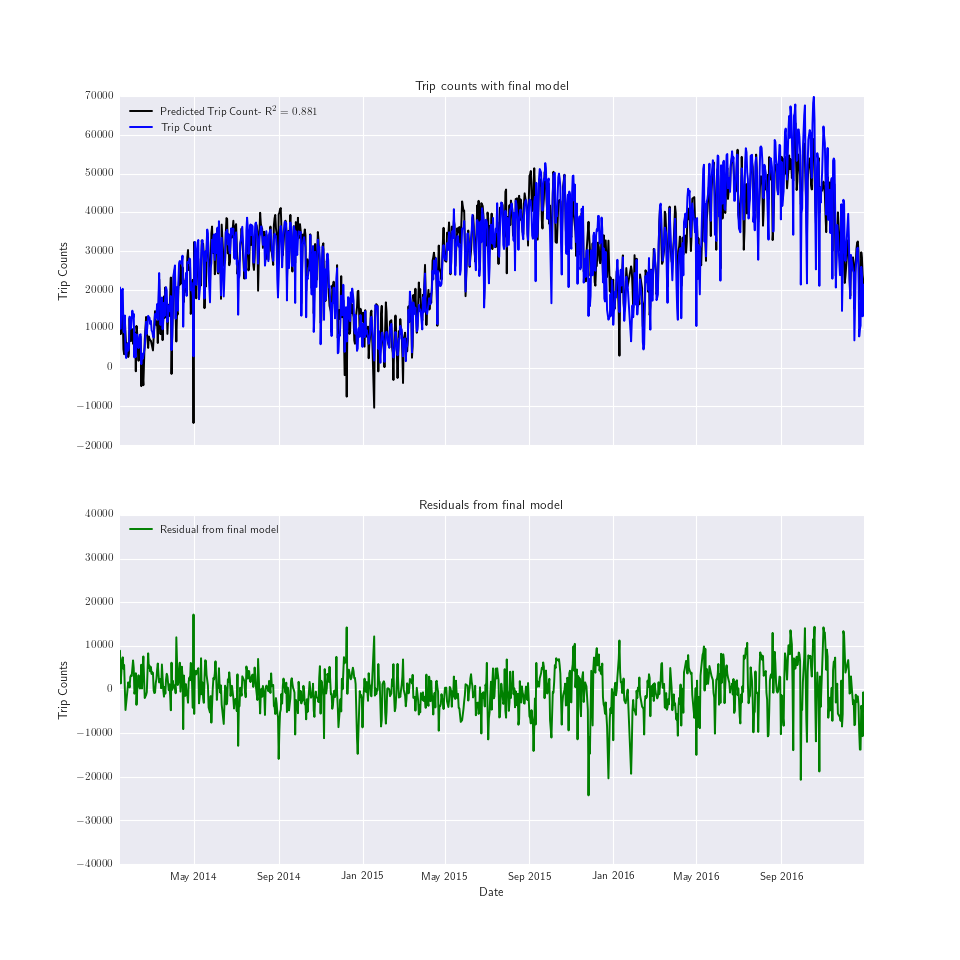
\includegraphics[width=\textwidth]{figures/final_plot.png}
\end{figure}
  
 \section{Results and Discussion}
 
To evaluate the models, we present $R^2$ values for the training and test sets:
\begin{center}
\begin{tabular} {| c | c | c |}
\hline
\textbf{Model} & \textbf{Train} & \textbf{Test} \\
\hline
\textbf{Baseline (Simple Linear)} &  \input{./../models/scores/lr_train_r2.txt} & \input{./../models/scores/lr_test_r2.txt} \\
\hline
\textbf{Final (Elastic Net)} &  \input{./../models/scores/EN_train_r2.txt} & \input{./../models/scores/EN_test_r2.txt} \\
\hline
\end{tabular}
\end{center}

Based on this training/test performance, we draw a couple of conclusions:
\begin{itemize}
\item The decrease in performance (for both models) from training to testing suggests overfitting. However, given the small sample size, it may also be random noise (due to the training/test split). With additional time, this could be explored further (for example by looking at the standard error in the estimated out-of-sample $R^2$ from cross-validation). 
\item Regardless, it is apparent that the final model is a dramatic improvement over the simple baseline in predicting the number of CitiBike rides taken on a given day.
\end{itemize}

\end{document}
